\chapter{Pesawat Sederhana: Tuas, Katrol, Bidang Miring}\label{ch:g5:simple-machines}

Tanpa mesin, tanpa listrik --- namun dengan beberapa balok, tali, dan
landasan miring, para pembangun zaman kuno mengangkat batu yang tidak
sanggup diseret sepasukan sapi. Kotak alat mereka berisi \emph{\omterm{def:g5:simple-machines:machine}{pesawat
sederhana}}: temuan yang sama sekali tidak bermotor, yang mengubah
tarikan lemah yang santai menjadi tarikan yang perkasa. Kamu sudah
memiliki yang pertama; berkenalanlah dengan keluarganya.

\section{Keluarga penghemat tenaga}

\begin{definition}[Pesawat sederhana]\label{def:g5:simple-machines:machine}
Sebuah \emph{pesawat sederhana}\index{pesawat sederhana} adalah alat
tanpa motor yang mengubah sebuah \omterm{def:g2:pushes-and-pulls:force}{gaya} agar sesuai bagi kita:
membuatnya lebih kuat, atau mengubah arahnya, atau keduanya. Yang
klasik: \emph{\omterm{def:g3:levers-and-scales:lever}{tuas}} yang kamu kenal dari jungkat-jungkit dan linggis,
\emph{\omterm{def:g5:simple-machines:pulley}{katrol}}, dan \emph{\omterm{def:g5:simple-machines:ramp}{bidang miring}} --- landasan miring yang
sederhana.
\end{definition}

\begin{example}[Tuas, ditinjau kembali]\label{ex:g5:simple-machines:lever}
Aturan \omterm{def:g3:levers-and-scales:lever}{tuas} sudah kamu miliki: koin dikali tanda --- gayamu yang kecil
jauh dari \omterm{def:g3:levers-and-scales:lever}{titik tumpu} mengalahkan beban besar yang dekat dengannya.
Perhatikan sesuatu yang lain sekarang: ujung linggismu menyapu jauh ke
bawah sementara bongkah batunya naik hanya sedikit. Simpanlah
pengamatan itu di sakumu; sebentar lagi ia menjadi sebuah hukum.
\end{example}

\section{Katrol}

\begin{definition}[Katrol]\label{def:g5:simple-machines:pulley}
Sebuah \emph{katrol}\index{katrol} adalah roda beralur tempat tali
duduk. Katrol \emph{tetap} tergantung pada sebuah balok dan hanya
mengubah arah tarikanmu: tariklah ke bawah, bebannya naik. Katrol
\emph{bergerak} menunggangi talinya dengan beban terkait padanya:
bebannya lalu tergantung pada \emph{dua} untai tali, dan tiap untainya
hanya membawa separuh \omterm{def:g4:weight-and-mass:weight}{beratnya}.
\end{definition}

\begin{omfigure}
\begin{tikzpicture}[scale=0.8]
  \draw[thick] (0.2,4.4) -- (2.8,4.4);
  \draw[thick] (1.5,4.4) circle (0.42);
  \draw[thick] (1.08,4.4) -- (1.08,1.6);
  \draw[thick] (1.92,4.4) -- (1.92,2.8);
  \draw[thick, fill=omMeth, fill opacity=0.4]
    (0.68,0.8) rectangle (1.48,1.6);
  \node[font=\footnotesize] at (1.08,1.2) {beban};
  \draw[-Stealth, very thick, omThm] (1.92,2.8) -- (1.92,1.9);
  \node[right, font=\small] at (2.1,2.3) {tarikan penuh, ke bawah};
  \node[below, font=\small] at (1.5,0.3) {tetap: mengubah arah};
  \begin{scope}[xshift=6.6cm]
    \draw[thick] (0.2,4.4) -- (3.6,4.4);
    \draw[thick] (0.9,4.4) -- (0.9,2.2);
    \draw[thick] (1.74,2.2) circle (0.42) ;
    \draw[thick] (0.9,2.2) arc (180:360:0.42);
    \draw[thick] (2.58,2.2) -- (2.58,4.4);
    \draw[thick] (2.58,3.4) -- (2.58,4.4);
    \draw[thick] (1.74,1.78) -- (1.74,1.5);
    \draw[thick, fill=omMeth, fill opacity=0.4]
      (1.34,0.7) rectangle (2.14,1.5);
    \node[font=\footnotesize] at (1.74,1.1) {beban};
    \draw[-Stealth, very thick, omThm] (2.58,4.4) -- (2.58,4.9);
    \node[right, font=\small] at (2.75,4.6) {separuh tarikan};
    \node[below, font=\small] at (1.9,0.3)
      {bergerak: dua untai berbagi beban};
  \end{scope}
\end{tikzpicture}

{\small Dua \omterm{def:g5:simple-machines:pulley}{katrol}, dua hadiah. \omterm{def:g5:simple-machines:pulley}{Katrol} tetap memutar arah tarikanmu;
\omterm{def:g5:simple-machines:pulley}{katrol} bergerak membuat dua untai tali berbagi bebannya, sehingga
tanganmu hanya menahan separuhnya.}
\end{omfigure}

\begin{omfigure}
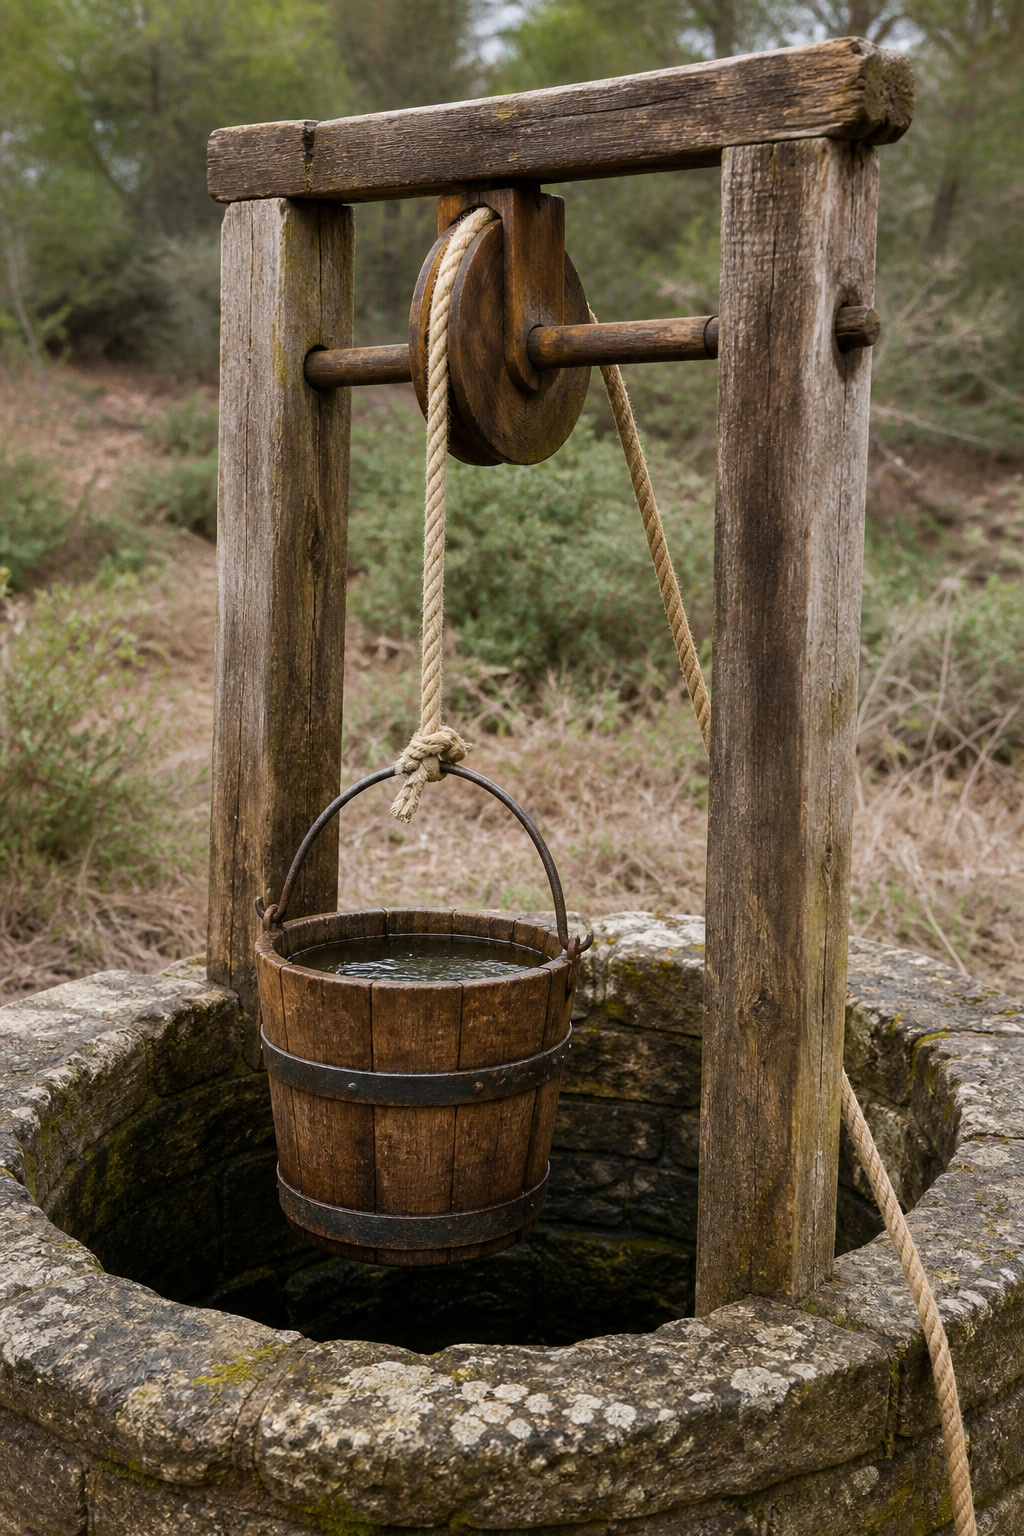
\includegraphics[width=0.34\linewidth]{images/book1/ai/g5-machines-pulley.jpg}

{\small \omterm{def:g5:simple-machines:pulley}{Katrol} sumur: talinya duduk di dalam alurnya, dan tarikan ke bawah menjadi angkatan ke atas.}
\end{omfigure}

\begin{example}[Katrol yang bekerja]\label{ex:g5:simple-machines:pulleywork}
Bendera naik di tiangnya sementara tanganmu menarik dengan santai
\emph{ke bawah}: itu \omterm{def:g5:simple-machines:pulley}{katrol} tetap di puncaknya --- arahnya berubah,
tenaganya tidak, tetapi menarik ke bawah membuat beratmu sendiri ikut
menolong. Kerekan majemuk tukang bangunan merangkai beberapa \omterm{def:g5:simple-machines:pulley}{katrol}
sehingga bebannya tergantung pada empat atau enam untai: tiap untai
membawa seperempat atau seperenam \omterm{def:g4:weight-and-mass:weight}{beratnya}, dan satu pekerja
mengangkat sebuah piano. Amatilah pekerjanya, namun: \omterm{def:g2:measuring-length:units}{meter} demi \omterm{def:g2:measuring-length:units}{meter}
tali berlari melewati tangannya, sementara pianonya sendiri merayap
naik pelan-pelan.
\end{example}

\section{Bidang miring}

\begin{definition}[Bidang miring]\label{def:g5:simple-machines:ramp}
Sebuah \emph{bidang miring}\index{bidang miring} --- sebuah landasan
miring --- adalah lereng untuk menaikkan beban tanpa mengangkatnya
lurus ke atas. Makin landai lerengnya, makin kecil dorongan yang
diperlukan untuk memindahkan bebannya di sepanjang lereng itu:
menggelindingkan tong ke atas landasan yang panjang dan landai itu
mudah; ke atas landasan yang pendek dan curam, \omterm{def:g4:weight-and-mass:weight}{berat} sekali; lurus ke
atas, mustahil.
\end{definition}

\begin{method}[Rasakan dengan neraca karet gelang]\label{met:g5:simple-machines:measure}
\omterm{def:g3:levers-and-scales:scale}{Neraca} karet gelangmu dari tahun lalu dapat mencicipi bedanya:
\begin{enumerate}
  \item naikkan mobil mainan ke atas sebuah papan lalu kaitkan karet
        gelangnya padanya;
  \item sandarkan papannya sebagai landasan landai pada tumpukan buku
        yang rendah; seretlah mobilnya pelan-pelan ke atas dengan
        karetnya lalu catat regangannya;
  \item sandarkan papan yang sama jauh lebih curam, pada dudukan
        kursi, lalu seret lagi.
\end{enumerate}
Seretan pada yang curam meregangkan karetnya jauh lebih jauh: makin
curam lerengnya, makin besar tenaganya. Lereng yang landai memang
benar-benar landai --- alatmu sendiri yang mengatakannya.
\end{method}

\begin{omfigure}
\begin{tikzpicture}[scale=0.8]
  \draw[thick] (0,0) -- (11.2,0);
  \draw[very thick, omDef] (0.3,0) -- (6.5,2.0);
  \draw[thick, fill=omMeth, fill opacity=0.4]
    (2.8,0.82) rectangle ++(0.8,0.55);
  \draw[-Stealth, thick, omThm] (3.75,1.35) -- (4.65,1.64);
  \node[above, font=\small, omThm] at (3.4,1.75) {dorongan kecil};
  \draw[very thick, omDef] (8.2,0) -- (10.2,2.0);
  \draw[thick, fill=omMeth, fill opacity=0.4]
    (8.75,0.5) rectangle ++(0.8,0.55);
  \draw[-Stealth, very thick, omThm] (9.75,1.25) -- (10.55,2.05);
  \node[above, font=\small, omThm] at (9.3,1.9) {dorongan besar};
  \node[below, font=\small] at (3.4,-0.3)
    {landasan panjang dan landai ke tinggi yang sama};
  \node[below, font=\small] at (9.3,-0.3) {landasan pendek dan curam};
\end{tikzpicture}

{\small Peti yang sama, tinggi yang sama untuk dicapai: landasan yang
panjang dan landai meminta dorongan kecil di sepanjang jalan yang
panjang; landasan yang curam, dorongan besar di jalan yang pendek.}
\end{omfigure}

\begin{example}[Bidang miring di sekitar kita]\label{ex:g5:simple-machines:ramps}
Landasan kursi roda dibuat panjang dan landai di sebelah tangga yang
pendek --- kelandaian yang disengaja. Jalan gunung berkelok-kelok:
alih-alih menyerang puncaknya lurus ke atas, jalan itu melilitkan
\omterm{def:g5:simple-machines:ramp}{bidang miring} yang panjang dan landai bolak-balik menyeberangi
lerengnya. Dan sekrup adalah \omterm{def:g5:simple-machines:ramp}{bidang miring} yang menyamar --- lereng
yang dililitkan pada sebatang tongkat, sehingga tiap putaran obeng
yang ringan menyelundupkan sekrupnya selangkah mungil lebih dalam.
\end{example}

\section{Aturan emas}

\begin{proposition}[Aturan emas pesawat]\label{prop:g5:simple-machines:golden}
Tidak ada \omterm{def:g5:simple-machines:machine}{pesawat sederhana} yang memberi sesuatu dengan cuma-cuma: apa
pun yang dihematnya pada \omterm{def:g2:pushes-and-pulls:force}{gaya}, ditagihnya kembali pada jarak. Separuh
\omterm{def:g2:pushes-and-pulls:force}{gaya} --- dua kali tali yang ditarik, atau dua kali jalan yang
ditempuh; sepersepuluh \omterm{def:g2:pushes-and-pulls:force}{gaya} --- sepuluh kali jalannya. Pesawat demi
pesawat, pertukarannya persis: kenyamanan dibeli dengan \omterm{def:g2:measuring-length:units}{meter}.
\end{proposition}

\begin{example}[Memeriksa aturannya]\label{ex:g5:simple-machines:check}
\omterm{def:g5:simple-machines:pulley}{Katrol} bergerak: tanganmu menarik dengan separuh \omterm{def:g2:pushes-and-pulls:force}{gaya}, dan untuk
menaikkan bebannya \qty{1}{m} kamu menarik masuk \qty{2}{m} tali ---
kedua untainya harus memendek satu \omterm{def:g2:measuring-length:units}{meter}. Linggis: ujungmu menyapu
busur yang panjang, bongkah batunya nyaris tidak bergeming. Landasan
miring: petinya mencapai tinggi yang sama, tetapi kamu mendorongnya di
sepanjang seluruh lerengnya. Setiap penghematan terbayar, dengan
persis.
\end{example}

\begin{remark}[Mengapa aturannya tidak dapat dicurangi]\label{rem:g5:simple-machines:whygolden}
Bersembunyi di bawah aturan emas ada kawan lama kita dari bab \omterm{def:g5:everyday-energy:energy}{energi}:
mengangkat beban sampai ketinggian tertentu memakan jatah \omterm{def:g5:everyday-energy:energy}{energi} yang
tetap, dan susunan tali serta papan apa pun tidak mengubah harganya.
Pesawat hanya membolehkanmu membayarnya dengan uang receh --- yang
lebih banyak jumlahnya. \omterm{def:g2:pushes-and-pulls:force}{Gaya} kecil di sepanjang jalan yang panjang
menyerahkan \omterm{def:g5:everyday-energy:energy}{energi} yang sama dengan gaya besar di jalan yang pendek.
Mesin abadi gagal justru karena ini: tagihannya selalu tagihan.
\end{remark}

\section{Latihan}

\begin{exercise}[$\star$]\label{exo:g5:simple-machines:1}
Sebutkan ketiga \omterm{def:g5:simple-machines:machine}{pesawat sederhana} yang klasik, dan satu tempat
sehari-hari untuk menemukan masing-masingnya.
\end{exercise}

\begin{exercise}[$\star$]\label{exo:g5:simple-machines:2}
Apa yang diubah \omterm{def:g5:simple-machines:pulley}{katrol} tetap pada tarikanmu? Apa yang diubah \omterm{def:g5:simple-machines:pulley}{katrol}
bergerak?
\end{exercise}

\begin{exercise}[$\star$]\label{exo:g5:simple-machines:3}
Mengapa menarik bendera \emph{ke bawah} untuk menaikkannya lebih
nyaman daripada mengangkat \omterm{def:g4:weight-and-mass:weight}{berat} yang sama lurus ke atas, padahal
tenaganya sama besar?
\end{exercise}

\begin{exercise}[$\star$]\label{exo:g5:simple-machines:4}
Dengan satu \omterm{def:g5:simple-machines:pulley}{katrol} bergerak, bebannya tergantung pada dua untai.
Berapa bagian dari \omterm{def:g4:weight-and-mass:weight}{beratnya} yang ditahan tanganmu? Untuk menaikkan
bebannya \qty{3}{m}, berapa panjang tali yang harus kamu tarik?
\end{exercise}

\begin{exercise}[$\star$]\label{exo:g5:simple-machines:5}
Pada \cref{met:g5:simple-machines:measure}, landasan mana yang
meregangkan karet gelangnya lebih jauh? Apa yang membayar regangan
yang lebih kecil pada landasan yang lebih landai?
\end{exercise}

\begin{exercise}[$\star$]\label{exo:g5:simple-machines:6}
Mengapa jalan gunung berkelok-kelok alih-alih berjalan lurus ke atas
lerengnya? \omterm{def:g5:simple-machines:machine}{Pesawat sederhana} yang mana yang diwujudkan seluruh jalan
itu?
\end{exercise}

\begin{exercise}[$\star$]\label{exo:g5:simple-machines:7}
Nyatakan aturan emas pesawat. Sebuah pesawat membuatmu dapat menarik
dengan sepersepuluh \omterm{def:g2:pushes-and-pulls:force}{gaya} --- apa yang ditagihnya kepadamu?
\end{exercise}

\begin{exercise}[$\star$]\label{exo:g5:simple-machines:8}
Bagaimana sekrup menjadi \omterm{def:g5:simple-machines:ramp}{bidang miring} yang menyamar? Apa yang
berperan sebagai jalan panjang yang landai?
\end{exercise}

\begin{exercise}[$\star\star$]\label{exo:g5:simple-machines:9}
Sebuah kerekan majemuk menggantungkan piano pada empat untai. Berapa
bagian dari \omterm{def:g4:weight-and-mass:weight}{berat} pianonya yang ditarik tangan pekerjanya? Untuk
menaikkan pianonya \qty{2}{m}, berapa \omterm{def:g2:measuring-length:units}{meter} tali yang melewati
tangannya?
\end{exercise}

\begin{exercise}[$\star\star$]\label{exo:g5:simple-machines:10}
Sebuah landasan bongkar muat panjangnya \qty{6}{m} dan naik
\qty{1}{m}; mendorong peti ke atasnya memerlukan dorongan yang sedang.
Para pengangkut yang tidak sabar memotong landasan baru yang
panjangnya hanya \qty{3}{m} ke peron yang sama. Dengan aturan emas,
bandingkan dorongan yang baru dengan yang lama --- dan jelaskan
mengapa ``separuh jalan'' bukanlah tawaran yang menguntungkan.
\end{exercise}

\begin{exercise}[$\star\star$]\label{exo:g5:simple-machines:11}
Sebuah iklan menawarkan seperangkat \omterm{def:g5:simple-machines:pulley}{katrol} ``yang begitu cerdik
sehingga kamu menarik satu \omterm{def:g2:measuring-length:units}{meter} tali dengan separuh \omterm{def:g2:pushes-and-pulls:force}{gaya} --- dan
bebannya naik satu \omterm{def:g2:measuring-length:units}{meter} penuh''. Adililah pernyataan itu di hadapan
aturan emas dan tagihan \omterm{def:g5:everyday-energy:energy}{energi} pada
\cref{rem:g5:simple-machines:whygolden}: adakah susunan roda dan tali
mana pun yang dapat memenuhinya?
\end{exercise}
